\chapter{Manual de Usuario}\label{manual}

Al acceder a la dirección TODO nos encontraremos con la siguiente pantalla:\\

\figura{1}{img/cap9/1-inicio-not-logged.png}{Inicio}{fig:inicionl}{}

Aunque muchas de las funciones de la aplicación son accesibles sin necesidad de disponer de una cuenta en la misma, primero procederemos al registro para poder así ver la funcionalidad completa de la aplicación.\\

Para registrarnos, hacemos click en el botón de ``Empieza ya", {(v\'ease la figura~\ref{fig:inicionl})} lo que nos llevará a la pantalla de registro.\\

\clearpage

\figura{0.9}{img/cap9/2-registro.png}{Registro}{fig:registro}{}

Una vez rellenamos los datos de manera correcta, hacemos click en el botón ``Regístrate",{(v\'ease la figura~\ref{fig:registro})} y si todo ha ido bien, nos devolverá a la página de inicio, pero esta vez con nuestra cuenta creada y la sesión iniciada.{(v\'ease la figura~\ref{fig:iniciol})}\\

\figura{0.9}{img/cap9/3-inicio-logged.png}{Inicio con sesión iniciada}{fig:iniciol}{}

\clearpage

Desde el inicio tenemos acceso a la mayoría de catálogos de la aplicación. Si nos vamos, por ejemplo, al catálogo de peces, veremos la siguiente pantalla.{(v\'ease la figura~\ref{fig:catpeces})}\\

\figura{0.9}{img/cap9/4-catalogo-peces.png}{Catálogo peces}{fig:catpeces}{}

Aquí, al igual que en todos los catálogos, disponemos de unos filtros para poder realizar una búsqueda algo más precisa. En el caso de los peces, podemos filtrar por el tamaño de su sombra, por los lugares en los que podemos encontrarlos y por su nombre. En el caso de haber iniciado sesión podemos filtrar por aquellos peces que hemos obtenido ya o no.\\

En la gran mayoría de catálogos, hay un botón de check para que el usuario pueda ir indicando si ha obtenido el pez o no {(v\'ease la figura~\ref{fig:pecesobtenidos})}. De esta forma puede llevar un recuento de aquellos peces que ya ha obtenido para ir completando su colección.\\

\figura{0.9}{img/cap9/5-peces-obtenidos.png}{Peces obtenidos}{fig:pecesobtenidos}{}

\clearpage

Además, podemos hacer click en las fotos de los peces para obtener información sobre los mismos, como el lugar y la hora donde se puede obtener, así como otros datos. Adicionalmente, podemos ver los meses en los que el pez está disponible tanto para el hemisferio norte como para el hemisferio sur si hacemos click en el botón superior izquierda {(v\'eanse las figuras~\ref{fig:infonorte} y ~\ref{fig:infosur})}.\\

\begin{figure}[!htb]
	\begin{minipage}{0.48\textwidth}
		\centering
		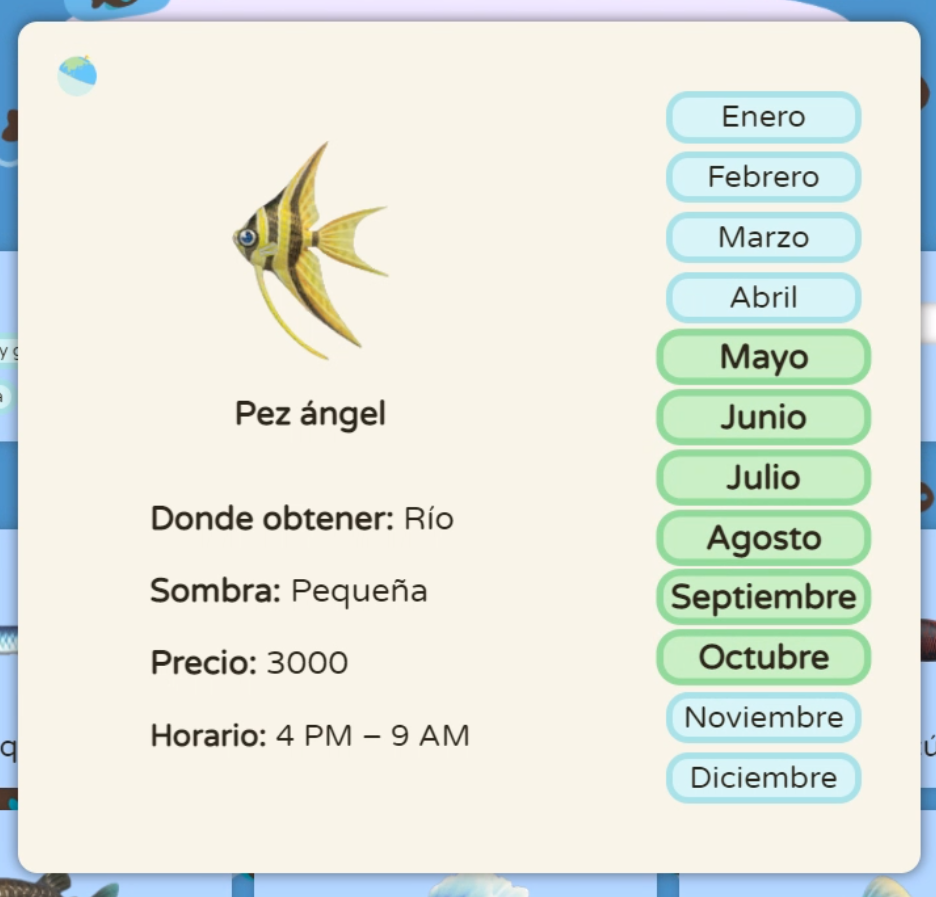
\includegraphics[width=.9\linewidth]{img/cap9/6-pez-info-norte.png}
		\caption{Info hemisferio norte}
		\label{fig:infonorte}
	\end{minipage}\hfill
	\begin{minipage}{0.48\textwidth}
		\centering
		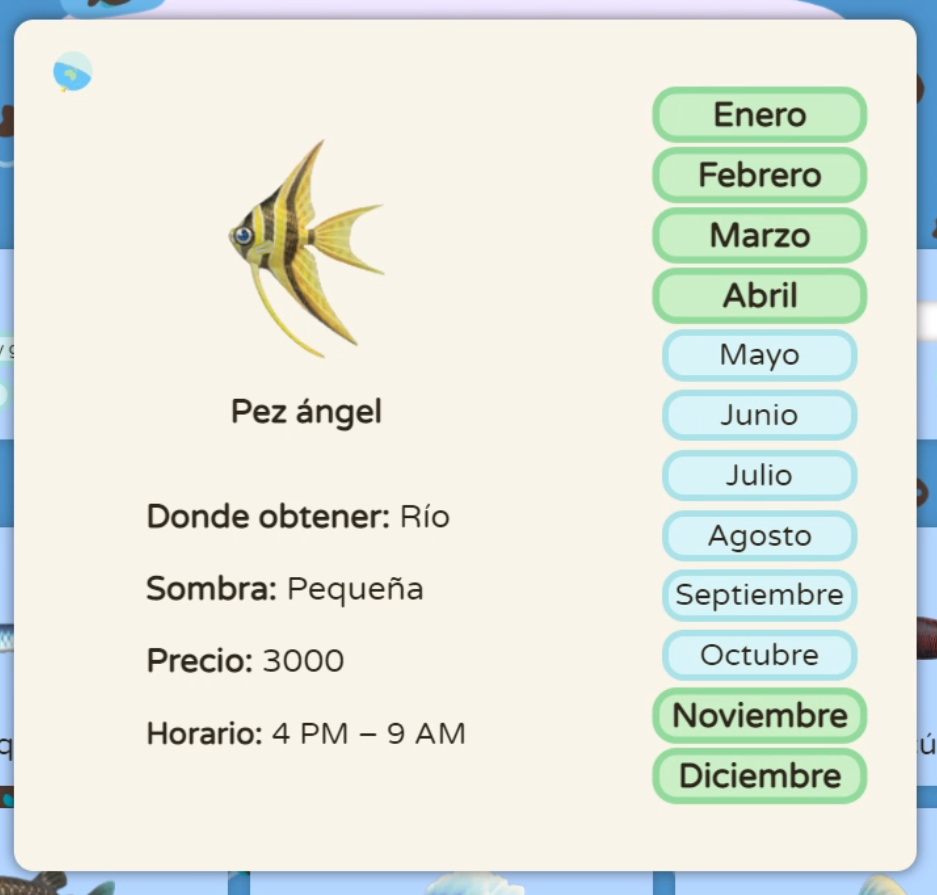
\includegraphics[width=.9\linewidth]{img/cap9/7-pez-info-sur.png}
		\caption{Info hemisferio sur}
		\label{fig:infosur}
	\end{minipage}
\end{figure}

Además, tenemos la opción de navegar por las distintas páginas de los resultados, bien avanzando o retrocediendo de uno en uno con los botones de las flechas, o bien haciendo click sobre la página deseada {(v\'ease la figura~\ref{fig:paginacion})}.\\

\figura{0.7}{img/cap9/8-paginacion.png}{Paginación}{fig:paginacion}{}

\clearpage

De la misma forma, la gran mayoría de catálogos funcionan de manera idéntica con ciertas diferencias, como obviamente, la información que se muestra al hacer click en un ítem. Hay otros cambios en algunos catálogos, como en el de obras de arte, en el cual podemos observar que hay ciertas piezas con un botón, que indica que esa obra tiene una falsificación {(v\'ease la figura~\ref{fig:catarte})}.\\

\figura{0.7}{img/cap9/9-cat-arte.png}{Catálogo obras de arte}{fig:catarte}{}

Si hacemos click en ese botón, podemos ver un menú de información con las imágenes, tanto de la versión real como de la falsificación, para intentar ayudar al usuario a diferenciarlas {(v\'ease la figura~\ref{fig:falsificacion})}.\\

\figura{0.7}{img/cap9/10-falsificacion.png}{Falsificación}{fig:falsificacion}{}

\clearpage

Tanto en el catálogo de muebles como en el de ropa, existen ítems con variaciones {(v\'ease la figura~\ref{fig:variaciones})}. Estas variaciones podemos verlas desplazándonos con una barrita de desplazamiento y si hacemos click, veremos que cambia la imagen principal del ítem por el de la variante seleccionada {(v\'ease la figura~\ref{fig:variacion})}.\\

\begin{figure}[!htb]
	\begin{minipage}{0.48\textwidth}
		\centering
		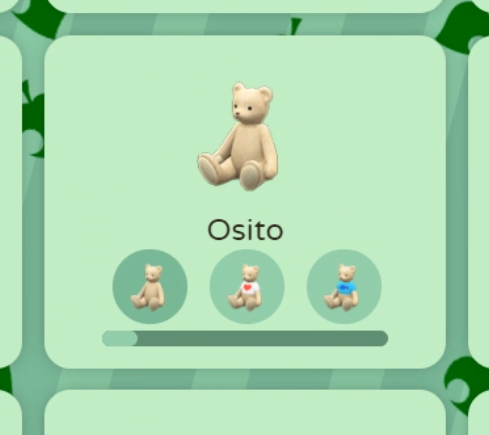
\includegraphics[width=.9\linewidth]{img/cap9/11-catalogo-muebles-variaciones.png}
		\caption{Variaciones}
		\label{fig:variaciones}
	\end{minipage}\hfill
	\begin{minipage}{0.48\textwidth}
		\centering
		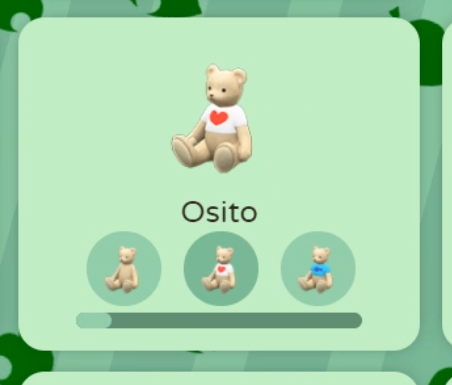
\includegraphics[width=.9\linewidth]{img/cap9/12-cat-muebles-variante.png}
		\caption{Variación}
		\label{fig:variacion}
	\end{minipage}
\end{figure}

En el catálogo de canciones, ademas de poder llevar recuento de aquellas canciones que hemos obtenido, podemos escucharlas. Si hacemos click en la imagen de la foto, esta empezará a reproducirse, y además disponemos de algunos controles en el reproductor abajo a la izquierda, tanto para pausar/continuar la canción como para ajustar el volumen {(v\'ease la figura~\ref{fig:catcancion})}.\\

\figura{0.8}{img/cap9/13-catalogo-canciones.png}{Catálogo canciones}{fig:catcancion}{}

\clearpage

Una vez terminado con los catálogos de la página de inicio, tenemos algunas otras herramientas accesibles desde la barra superior de navegación {(v\'ease la figura~\ref{fig:nav})}.\\

\figura{1}{img/cap9/14-nav.png}{Barra de navegación}{fig:nav}{}

Si hacemos click en la imagen de la izquierda, nos llevará a la página de inicio. Luego en la parte central disponemos de cuatro botones. El primero, ``Cazar ahora", nos lleva a un catálogo de los tres tipos de criaturas obtenibles, con la peculiaridad de que solo nos muestran aquellas criaturas capturables en la fecha y hora actuales {(v\'ease la figura~\ref{fig:cazarahora})}.\\

\figura{0.7}{img/cap9/15-cazar-ahora.png}{Cazar ahora}{fig:cazarahora}{}

Aquí, no solo disponemos de los filtros que tienen en su catálogo correspondiente, sino que además podemos cambiar el mes y hora, asi como el hemisferio (de manera global) para poder ver aquellas criaturas en función del mes y hora, de forma que le sea más sencillo al usuario y no tenga que dar vueltas por la isla sin saber qué o dónde se puede encontrar. Si hemos modificado el mes y/o la hora y deseamos volver a la actual, es tan fácil como hacer click en el botón de la flecha roja {(v\'ease la figura~\ref{fig:filtros})}.\\

\figura{0.9}{img/cap9/16-filtros-cazar-ahora.png}{Filtros}{fig:filtros}{}

Dentro de este catálogo, de base apareceremos en la pantalla de los insectos, por lo que si queremos ver los peces o las criaturas marinas es tan fácil como hacer click en el botón correspondiente a la derecha de los filtros.\\

\clearpage

Volviendo a la barra de navegación superior, el siguiente botón sería el de ``Sueños", pero para explicar por completo su funcionalidad necesitamos antes pasar por el perfil, por lo que se hablará de este catálogo más adelante. Por lo que primero haremos click en el botón que pone ``Mercado Nabos", que nos llevará a la siguiente pantalla {(v\'ease la figura~\ref{fig:mercadonabos})}.\\

\figura{0.9}{img/cap9/17-mercado-nabos.png}{Mercado nabos}{fig:mercadonabos}{}

En esta página podemos predecir tanto el precio de los nabos en la isla esta semana, así como el patrón que seguirá, y los posibles máximos y mínimos, todo para intentar sacar el mayor beneficio posible.\\

Para empezar, debemos rellenar tantos campos como podamos. El primero indica si es la primera vez que el usuario compra nabos o no, ya que la primera vez siempre se obtiene el mismo patrón.
El segundo botón indica el patrón de la semana anterior, que también dispone de un botón en caso de que el usuario no lo sepa. Por último, hay que indicar el precio al que se compraron los nabos el domingo {(v\'ease la figura~\ref{fig:datos})}.\\

\figura{1}{img/cap9/18-datos-nabos.png}{Datos}{fig:datos}{}

\clearpage

A partir de aquí, hay que indicar el precio al que Tendo y Nendo compran los nabos, tanto por la mañana como por la tarde. A mayor datos se introduzcan, mas precisa será la predicción. Como podemos ver, indicando los tres primeros campos, así como los precios del lunes, ya obtenemos una predicción bastante segura {(v\'ease la figura~\ref{fig:tablaprediccion})}.\\

\figura{0.7}{img/cap9/19-tabla-prediccion.png}{Tabla predicción}{fig:tablaprediccion}{}

Como podemos observar, se nos indica una fila por cada posible ``ruta" que puede suceder esa semana. A la izquierda vemos el patrón que podemos obtener, seguido de dos porcentajes que indican, el primero la probabilidad del patrón, y el segundo la probabilidad de la ``ruta" dentro del patrón. Luego observamos los precios, tanto los indicados por el usuario como los posibles para el resto de la semana. Los distintos colores representan el beneficio que puede representar, siendo rojo el menor beneficio y el verde oscuro el mayor beneficio. Por último, las dos últimas columnas nos indican tanto el mínimo garantizado como el máximo potencial al que se puede llegar.\\

Por ejemplo, si nos fijamos en la tabla, vemos que hay un 100\% de probabilidades de que esta semana obtengamos un patrón ``Pico pequeño", dentro del cual, a falta de más datos, tenemos seis posibles ``rutas" las cuales tienen todas la misma probabilidad de ocurrir. Sin embargo, todas tienen el mismo mínimo y máximo, siendo 139 y 200 bayas respectivamente.\\ 

\figura{0.8}{img/cap9/20-tabla-precisa.png}{Predicción precisa}{fig:prediccionprecisa}{}

Si rellenamos más datos a lo largo de la semana, vemos que se van reduciendo el número de filas ya que la predicción es mas precisa. Una vez rellenado los datos hasta la mitad del jueves, observamos que efectivamente, el patrón de esta semana es el ``Pico pequeño", que el mínimo y  máximo son los comentados anteriormente y que, el beneficio lo obtendremos entre la segunda mitad del jueves al sábado {(v\'ease la figura~\ref{fig:prediccionprecisa})}.\\

\clearpage

Obviamente, al ser datos ficticios no representa al 100\% la precisión de la herramienta, pero con datos reales obtenidos del juego que resulten mas coherentes con el algoritmo establecido dentro del juego, se pueden obtener resultados bastante precisos.\\

\figura{0.9}{img/cap9/21-info-nabos.png}{Información mercado}{fig:infomercado}{}

Si bajamos un poco, veremos que el usuario dispone de información para aprender cómo funciona el mercado de nabos dentro del juego, así como los posibles patrones que existen {(v\'ease la figura~\ref{fig:infomercado})}. Si coloca el cursor encima de cualquiera de las tarjetas de los patrones, podrá ver que aparece una breve descripción del funcionamiento del patrón en cuestión {(v\'ease la figura~\ref{fig:infopatrones})}. De esta forma, el usuario puede acceder a esta información para intentar rellenar los datos de la manera más precisa posible, obteniendo así un mejor resultado.\\

\figura{0.9}{img/cap9/22-info-patrones.png}{Información patrones}{fig:infopatrones}{}

\clearpage

La siguiente parada dentro de la barra de navegación superior sería el ``Calendario", el cual nos llevará a la siguiente pantalla al hacer click en él.\\

\figura{0.9}{img/cap9/23-calendario.png}{Calendario}{fig:calendario}{}

En esta pantalla disponemos de un calendario por el que podemos navegar, en el cuál se nos indican los eventos disponibles, siendo estos los cumpleaños de los distintos vecinos, así como otros eventos más especiales {(v\'ease la figura~\ref{fig:calendario})}. En azul clarito se resalta el día en el que nos encontramos, y si colocamos el cursor sobre cualquiera de los iconos situados en la parte inferior izquierda de cada día, podremos ver el título del evento. Si se trata de un cumpleaños, la celda obtendrá un color verde {(v\'ease la figura~\ref{fig:cumpleanos})}, mientras que si se trata de otro tipo de evento, tendrá un color distinto.\\

\figura{0.9}{img/cap9/24-calendario-cumple.png}{Cumpleaños}{fig:cumpleanos}{}

\clearpage

Si por ejemplo nos vamos al 31 de octubre, veremos que el icono corresponde a uno de los NPCs del juego, y al colocar el cursor sobre el, no solo nos indica que se trata de Halloween, sino que la celda obtiene un color anaranjado {(v\'ease la figura~\ref{fig:evento})}.\\

\figura{0.9}{img/cap9/25-calendario-halloween.png}{Evento}{fig:evento}{}

 Si en este caso (tratándose de un evento especial), hacemos click en el icono, se nos abrirá un menú con información del evento {(v\'ease la figura~\ref{fig:halloween})}.\\

\figura{0.9}{img/cap9/26-evento-halloween.png}{Halloween}{fig:halloween}{}

\clearpage

A continuación, como podemos ver en la barra de navegación, a la derecha del todo tenemos nuestro nombre de usuario seguido de una foto. Si hacemos click en la foto se nos abrirá un menú desplegable que nos da la opción de, o ir a nuestro perfil, o cerrar sesión {(v\'ease la figura~\ref{fig:navperfil})}.\\

\figura{0.9}{img/cap9/27-nav-perfil.png}{Desplegable perfil}{fig:navperfil}{}

En este caso haremos click en el botón ``Perfil", que nos llevará tal y como indica su nombre, a nuestro perfil {(v\'ease la figura~\ref{fig:perfil})}.\\

\figura{0.6}{img/cap9/28-perfil.png}{Perfil}{fig:perfil}{}

Observemos primero el menú de la izquierda. Representa el pasaporte del usuario, donde podremos ver la información proporcionada en el registro, así como el signo del zodiaco al que pertenece. Si el usuario quisiera modificar los datos, sería tan sencillo como hacer click en el lápiz azul del pasaporte, lo que nos llevaría al modo edición del mismo {(v\'ease la figura~\ref{fig:editarperfil})}.\\

\figura{0.7}{img/cap9/29-pasaporte-editando.png}{Editar perfil}{fig:editarperfil}{}

\clearpage

Una vez en dicho modo edición, podemos cambiar los datos a nuestro antojo, siempre y cuando cumplan los criterios de validación. Una vez listo, hacemos click en el botón del check verde para confirmar la operación. En caso de querer cancelar la operación, es tan fácil como volver a dejar los datos como estaban y hacer click en el check verde.\\

\figura{0.7}{img/cap9/30-pasaporte-updated.png}{Perfil actualizado}{fig:perfilactualizado}{}

Como podemos ver, se ha actualizado la información y además se ha cambiado el color de fondo del pasaporte {(v\'ease la figura~\ref{fig:perfilactualizado})}. El fondo varía de forma aleatoria tanto al acceder al perfil como al actualizar la información.\\

Ahora fijémonos en el menú que se encuentra a la derecha. Ahí podemos encontrar dos de las herramientas más importantes y útiles para el usuario. En primer lugar, se trata de las tareas personales. Al acceder al perfil por primera vez se encontrará vacío, como es nuestro caso. Sin embargo, haciendo click en el lápiz que encontramos a la derecha de dicho menú, entramos en el modo edición del mismo.\\

\figura{0.7}{img/cap9/31-tareas-edicion.png}{Modo edición}{fig:modoedicion}{}

Como podemos observar, ha aparecido un botón amarillo con un '+', {(v\'ease la figura~\ref{fig:modoedicion})}. Si hacemos click en ese botón, se nos creará una tarea nueva. Podemos crear hasta un máximo de 10 tareas, de forma que cuando creemos la décima ya no aparecerá el botón de crear. A continuación vamos a crear tres tareas.\\

\clearpage

\figura{0.7}{img/cap9/32-tres-tareas.png}{Nuevas tareas}{fig:nuevastareas}{}

Una vez creadas las tareas {(v\'ease la figura~\ref{fig:nuevastareas})}, estando en el modo edición, si hacemos click en cualquiera de las tareas, se nos abre el menú para personalizar la tarea {(v\'ease la figura~\ref{fig:menutareas})}. Aquí podemos, o bien cambiarle el icono a la tarea (ya que por defecto trae el de la hoja) haciendo click en el botón ``Actualizar" tras haber escogido otro icono, o bien borrarla haciendo click en el icono de la papelera. Para cerrar el menú es tan fácil como hacer click fuera del menú o deslizarnos en la página. Por ejemplo, vamos a cambiarle el icono a las dos primeras tareas y vamos a borrar la última.\\

\begin{figure}[!htb]
	\begin{minipage}{0.48\textwidth}
		\centering
		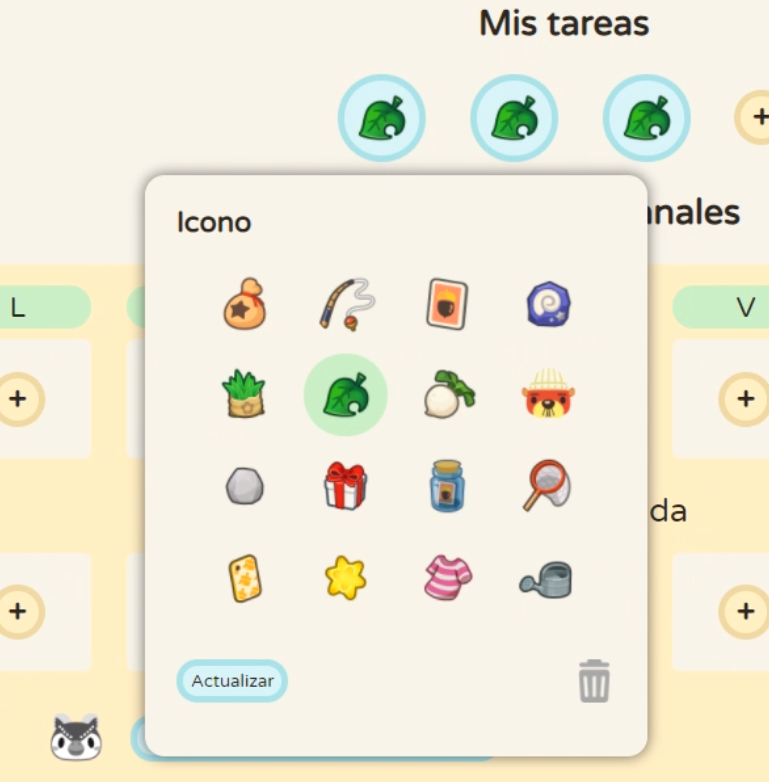
\includegraphics[width=.6\linewidth]{img/cap9/33-menu-tareas.png}
		\caption{Menú tareas}
		\label{fig:menutareas}
	\end{minipage}\hfill
	\begin{minipage}{0.48\textwidth}
		\centering
		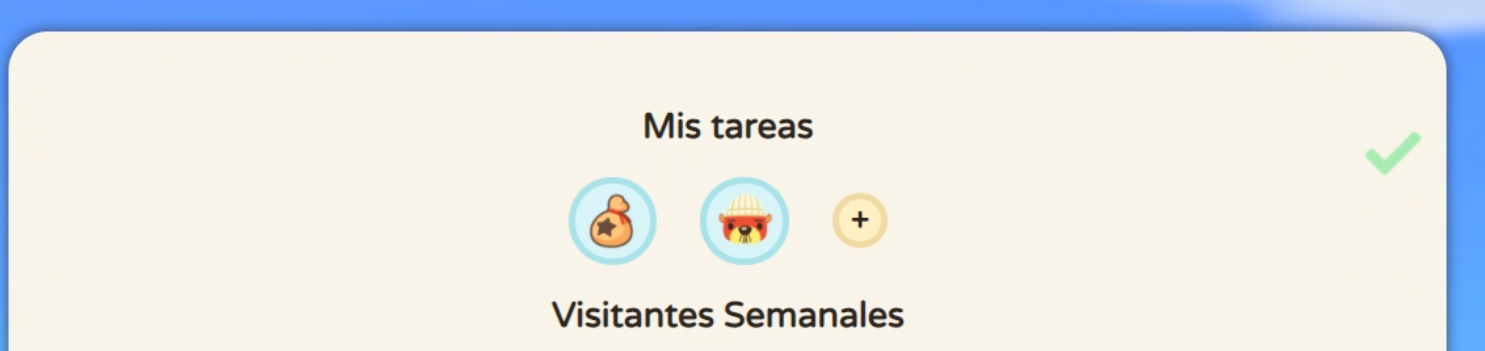
\includegraphics[width=\linewidth]{img/cap9/34-dos-tareas.png}
		\caption{Tareas editadas}
		\label{fig:tareaseditadas}
	\end{minipage}
\end{figure}

Una vez hayamos terminado, hacemos click en el check verde para salir del menú de edición {(v\'ease la figura~\ref{fig:tareaseditadas})} y ahora podemos activar o desactivar las tareas. Si hacemos click en cualquier tarea, se activará, cambiando su color a verde {(v\'ease la figura~\ref{fig:tarearealizada})}. Si volvemos a hacer click, se desactivará cambiando a azul. Si tenemos tareas activadas, al final del día se reiniciarán, ya que representan tareas diarias. De esta forma el usuario puede crear algunas tareas personalizables para representar su rutina en el juego, activarlas para recordar que ya la ha realizado y que se desactiven automáticamente para repetir el proceso cada día.\\

\figura{0.7}{img/cap9/35-tarea-done.png}{Tareas realizada}{fig:tarearealizada}{}

\clearpage

Ahora pasemos a la siguiente herramienta, los visitantes semanales. Aquí el usuario dispone de unos recuadros que representan tanto la semana actual como la anterior {(v\'ease la figura~\ref{fig:visitantessemanales})}. Los recuadros correspondientes al Sábado y Domingo son inalterables ya que, con ciertas excepciones debido a torneos puntuales, siempre van a venir los mismos visitantes durante esos días.\\

\figura{0.9}{img/cap9/36-visitantes-semanales.png}{Visitantes semanales}{fig:visitantessemanales}{}

En el resto de recuadros, si hacemos click en el botón de añadir, se nos abre un menú en el que veremos una lista de los posibles visitantes. Dependiendo de los que ya nos hayan visitado, acorde con cómo funciona en el juego, habrá algunos iconos que no se podrán seleccionar ya que habrán alcanzado su límite. Como máximo, solo se puede repetir un visitante en dos semanas conjuntas. Para mostrarlo, procedemos a rellenar los recuadros tal y como se ve en la imagen {(v\'ease la figura~\ref{fig:semanarellena})}.\\

\figura{0.9}{img/cap9/37-semana-rellena.png}{Semana rellanda}{fig:semanarellena}{}

\clearpage

Si volvemos a hacer click en cualquiera de los botones de añadir, veremos que los visitantes de la semana pasada, así como Alcatifa, que ya nos ha visitado en las dos semanas, serán menos visibles y no podrán seleccionarse {(v\'ease la figura~\ref{fig:menuvisitantes})}.\\

\figura{0.8}{img/cap9/38-menu-visitantes.png}{Menú visitantes}{fig:menuvisitantes}{}

En caso de querer modificar un visitante o eliminarlo, es tan fácil como hacer click en su icono y, o bien cambiarlo por otro, o bien hacer click en el icono de la papelera. Además, en la parte inferior de la herramienta podemos ver que hay un botón con el icono de Estela. Si hacemos click en él, podremos alternar entre dos estados, para indicar así si ya ha venido Estela esta semana a la isla.\\

Una vez hayamos modificado los datos, veremos que el icono de guardar (el check verde) empieza a parpadear. Esto significa que tenemos cambios sin guardar, por lo que para guardar los datos hay que hacer click. Si todo ha ido bien, veremos un mensaje confirmando que se ha guardado correctamente {(v\'ease la figura~\ref{fig:guardado})}.\\

\figura{0.9}{img/cap9/39-visitantes-guardados.png}{Confirmación guardado}{fig:guardado}{}

\clearpage

A continuación, seguimos con el siguiente apartado. Si deslizamos la página hacia abajo, veremos la siguiente sección del perfil: Mis vecinos. En este apartado, el usuario puede añadir los vecinos que estén en su isla. Al principio, si es una cuenta nueva, veremos diez recuadros solo con los botones para añadir {(v\'ease la figura~\ref{fig:misvecinos})}.\\

\figura{0.7}{img/cap9/40-vecinos-vacio.png}{Mis vecinos}{fig:misvecinos}{}

Para añadir un vecino, si hacemos click en cualquiera de los botones, se abrirá un menú en el que podremos buscar y seleccionar el vecino que deseemos. Una vez seleccionado, le damos al check verde para guardar los datos. Podremos ver como ahora aparece nuestro primer vecino, así como un corazón al lado. Este corazón indica la amistad que se tiene con el vecino, que por defecto viene a uno.\\

Ahora, si colocamos el cursor sobre el recuadro del vecino, podremos observar que se nos muestra a la izquierda un recuadro con información del mismo, así como su foto {(v\'ease la figura~\ref{fig:infovecino})}.\\

\figura{0.9}{img/cap9/41-info-vecino.png}{Información vecino}{fig:infovecino}{}

\clearpage

Si queremos cambiar o eliminar al vecino, es tan fácil como hacer click en su icono y volver a elegir otro y guardar, o a darle al botón de la papelera {(v\'ease la figura~\ref{fig:menuvecino})}. A continuación, vamos a añadir más vecinos para explicar con mas claridad el siguiente apartado.\\

\begin{figure}[!htb]
	\begin{minipage}{0.48\textwidth}
		\centering
		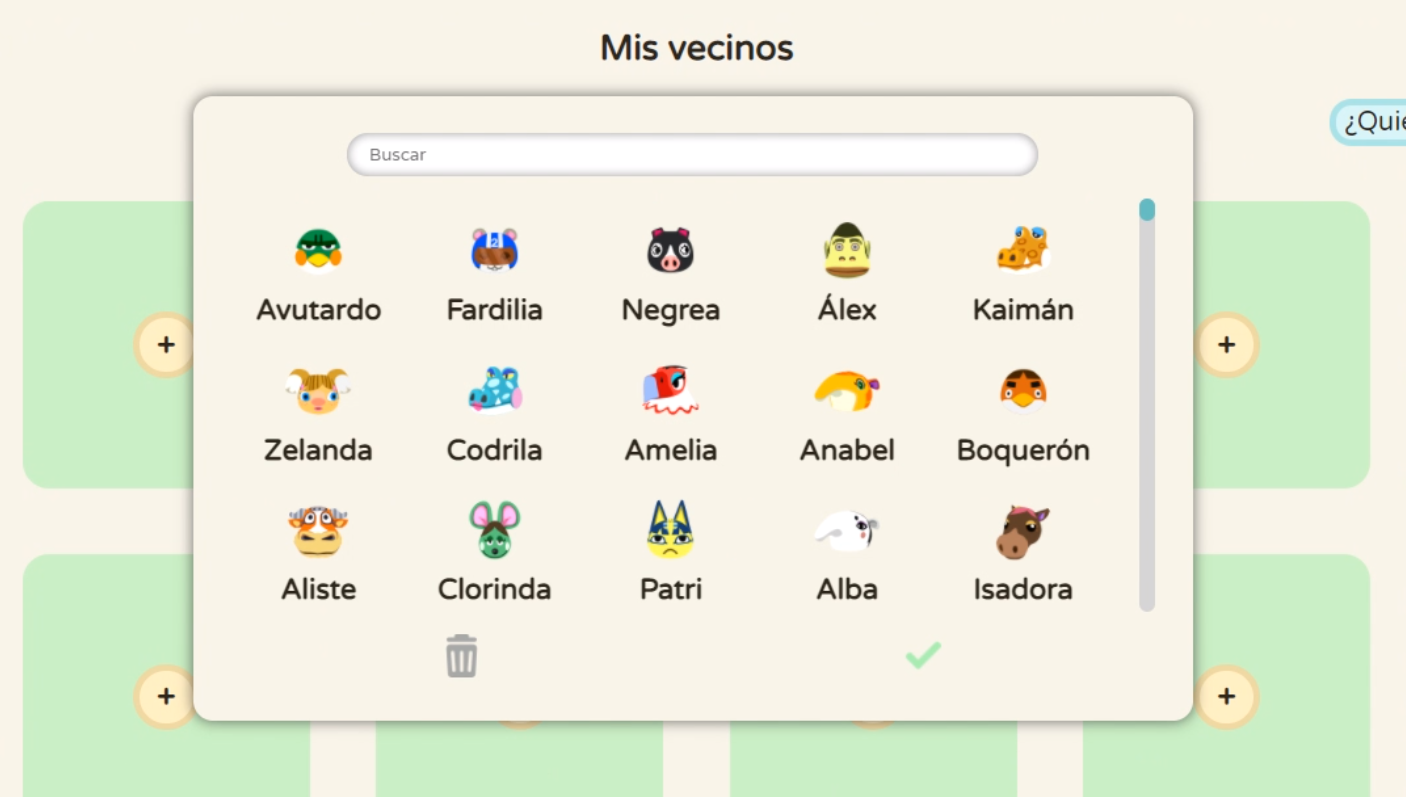
\includegraphics[width=.9\linewidth]{img/cap9/42-menu-vecinos.png}
		\caption{Menú vecinos}
		\label{fig:menuvecino}
	\end{minipage}\hfill
	\begin{minipage}{0.48\textwidth}
		\centering
		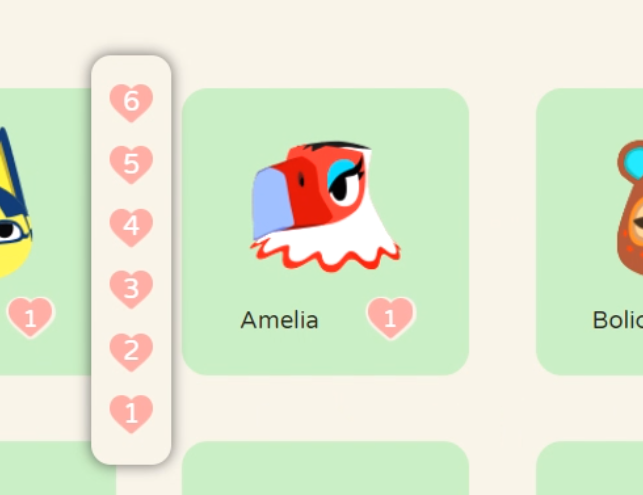
\includegraphics[width=.7\linewidth]{img/cap9/43-menu-amistad.png}
		\caption{Menú amistad}
		\label{fig:menuamistad}
	\end{minipage}
\end{figure}

Si hacemos click en el corazón de cada vecino, veremos que se nos abre un menú con seis corazones {(v\'ease la figura~\ref{fig:menuamistad})}. Aquí se puede cambiar el nivel de amistad del vecino haciendo click sobre el corazón con el número deseado.\\

Si nos fijamos, en la parte superior derecha de la herramienta podemos ver un botón azul. Si hacemos click en él, se nos abre un desplegable con información sobre el nivel de amistad de los vecinos, de forma que el usuario pueda saber qué nivel atribuir a cada vecino {(v\'ease la figura~\ref{fig:infoamistad})}.\\

\figura{0.9}{img/cap9/44-info-amistad.png}{Información amistad}{fig:infoamistad}{}

\clearpage

Además, en este desplegable vemos que hay un botón ``Calcular porcentaje". Si nos fijamos, en los recuadros han aparecido algunas cosas nuevas.\\

\figura{0.6}{img/cap9/45-porcentaje-mudanza-vacio.png}{Mudanza}{fig:mudanza}{}

Como vemos, cada vecino tiene un icono de bloquear, así como un pequeño recuadro azul {(v\'ease la figura~\ref{fig:mudanza})}. Esta sección sirve para calcular el porcentaje de mudanza de cada vecino, que tiene que ver con el nivel de amistad de cada uno. Siguiendo la información que podemos encontrar en el menú desplegable, podemos rellenar los niveles de amistad de cada vecino, así como excluirlos del cálculo si fuera necesario haciendo click en el botón de bloqueo. Si un vecino está siendo bloqueado, el icono aparecerá en rojo, y por lo tanto no contará para el cálculo de la probabilidad.\\

Una vez tengamos listo tanto la amistad, como aquellos vecinos bloqueados (en caso de haberlos), le damos al botón de ``Calcular porcentaje" que podemos encontrar más arriba. Podemos observar que han aparecido unos números en los recuadros azules {(v\'ease la figura~\ref{fig:calculoporcentaje})}, que indican la probabilidad que tiene cada vecino de mudarse de la isla. Como vemos, al haber bloqueado a Patri, esta no cuenta para el cálculo de la probabilidad y por lo tanto, no tiene número.\\

\figura{0.6}{img/cap9/47-porcentaje-mudanza.png}{Cálculo porcentaje}{fig:calculoporcentaje}{}

Tal y como funciona el juego, aquellos vecinos con mayor amistad tienen menos probabilidad de mudarse, por lo que, como podemos ver, Boliche que tiene un nivel seis de amistad (el máximo), es el que tiene menos probabilidades de mudarse (casi un 11\%), en comparación con Cacho y Lope, que al ser los que menos amistad tienen, hay más probabilidades de que sea uno de los dos el que decida mudarse (cada uno con casi un 34\% aproximadamente).\\

\clearpage

Una vez hayamos terminado, podemos volver a la vista original cerrando el menú desplegable haciendo click en el botón azul que se encuentra en la zona superior derecha del menú desplegable. Sigamos con la próxima herramienta, las Colecciones Especiales.\\

\figura{0.9}{img/cap9/48-colecciones-especiales.png}{Colecciones especiales}{fig:coleccesp}{}

Lo primero que nos encontramos es una serie de botones que indican la colección {(v\'ease la figura~\ref{fig:coleccesp})}. Una de ellas estará resaltada para denotar que es la colección activa. Si hacemos click en los distintos botones, vemos que los ítems de abajo van variando. Una vez hayamos seleccionado la colección deseada, podemos observar que hay varios ítems, cada uno con su imagen y nombre, así como un botón con forma de check gris. Si hacemos click en este botón, se volverá rojo indicando así que ya disponemos de este ítem {(v\'ease la figura~\ref{fig:checkobtenido})}.\\

Además, en caso de que sea necesario, hay botones para navegar por las paginas de ítems a los lados de la herramienta.\\

\figura{0.9}{img/cap9/49-coleccion-especial-check.png}{Check obtenido}{fig:checkobtenido}{}

\clearpage

Por último, tenemos el álbum de fotos del usuario{(v\'ease la figura~\ref{fig:album})}. Si hacemos click en el botón del menú de la derecha, nos aparecerá un menú para introducir la url de la imagen que queramos añadir a nuestro álbum {(v\'ease la figura~\ref{fig:aniadirimagen})}.\\

\begin{figure}[!htb]
	\begin{minipage}{0.48\textwidth}
		\centering
		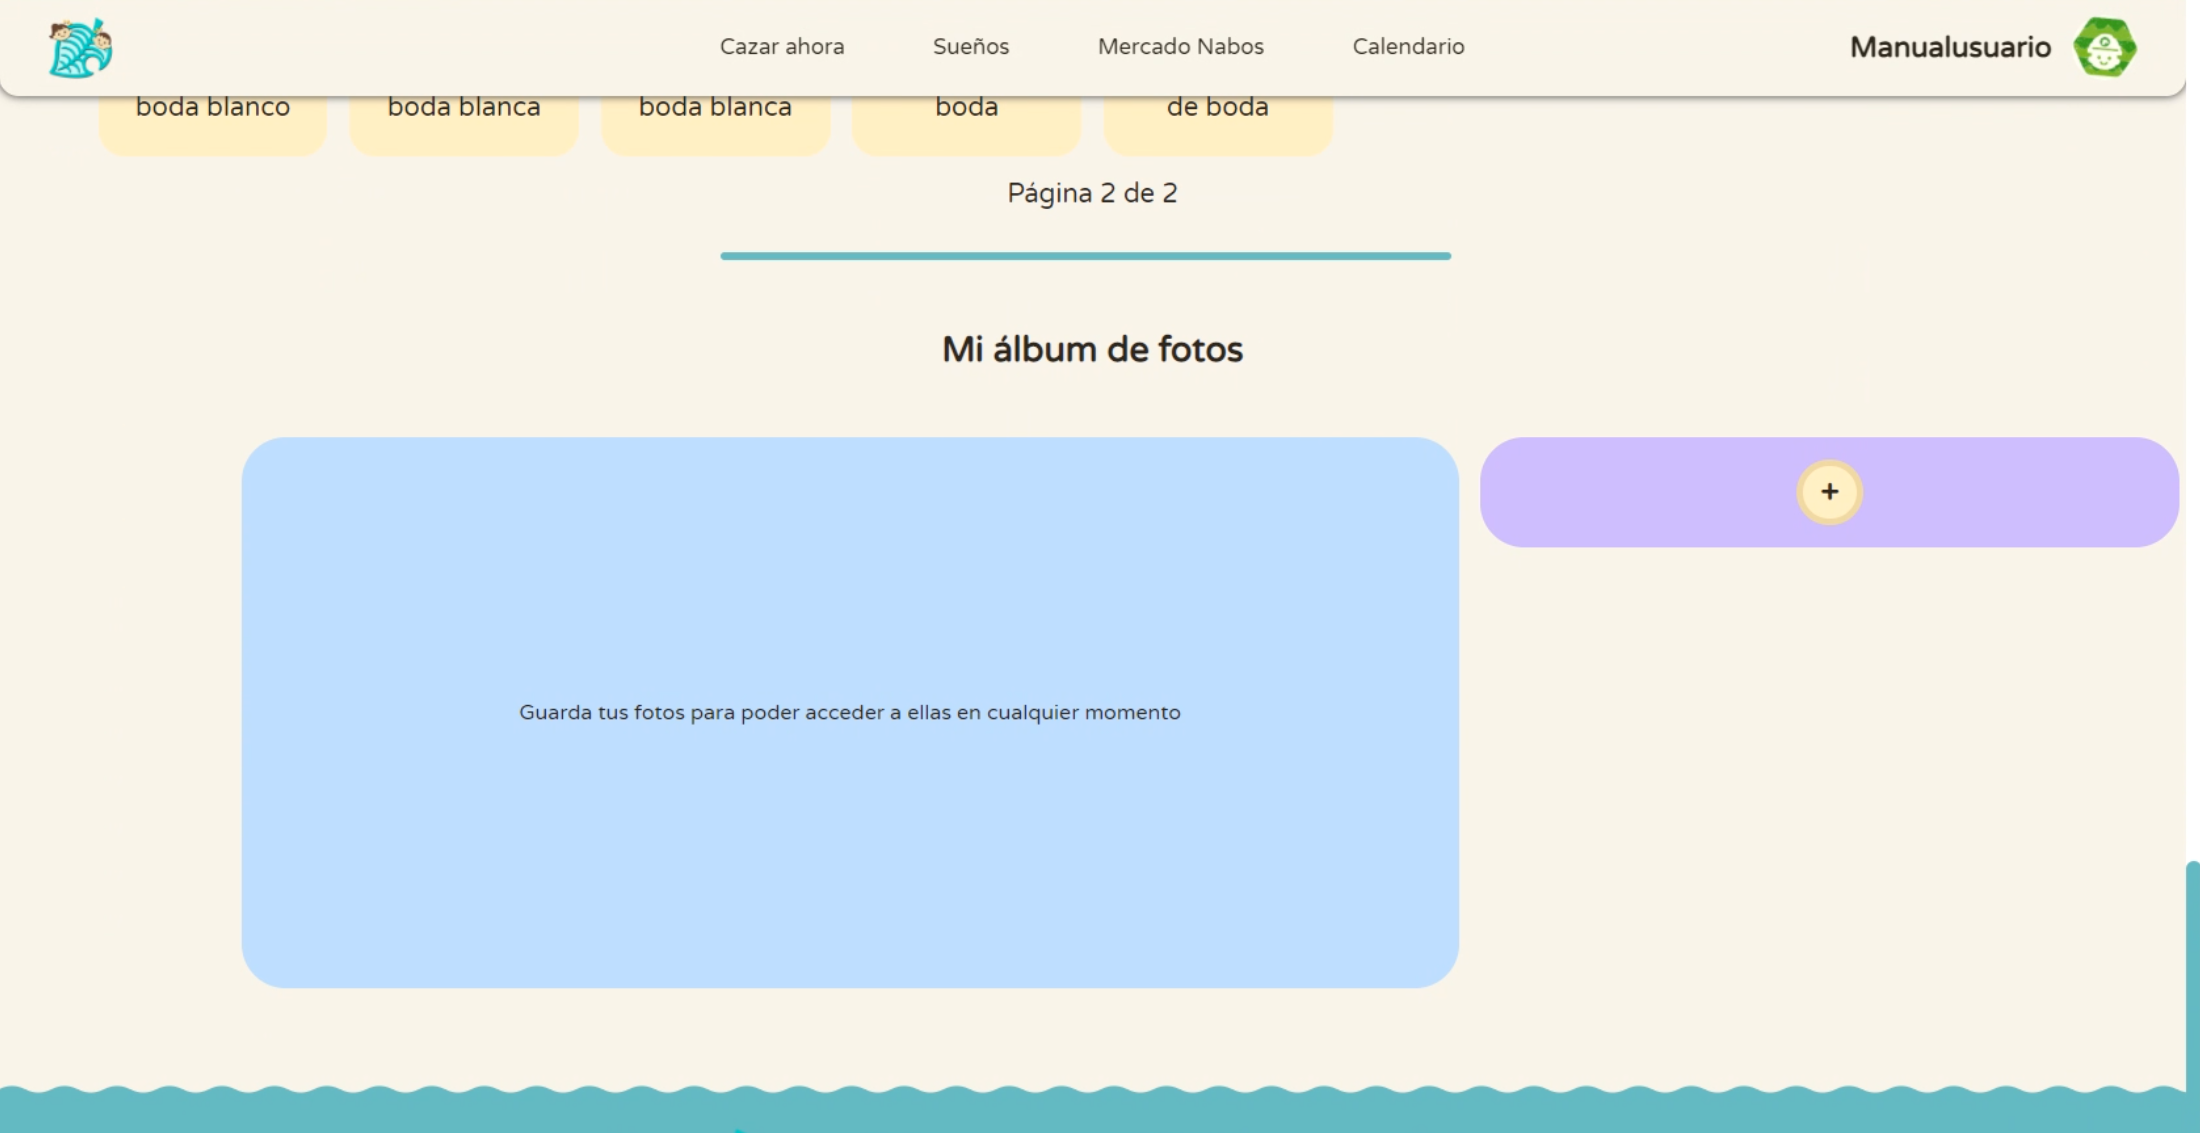
\includegraphics[width=.8\linewidth]{img/cap9/50-album-fotos.png}
		\caption{Álbum fotos}
		\label{fig:album}
	\end{minipage}\hfill
	\begin{minipage}{0.48\textwidth}
		\centering
		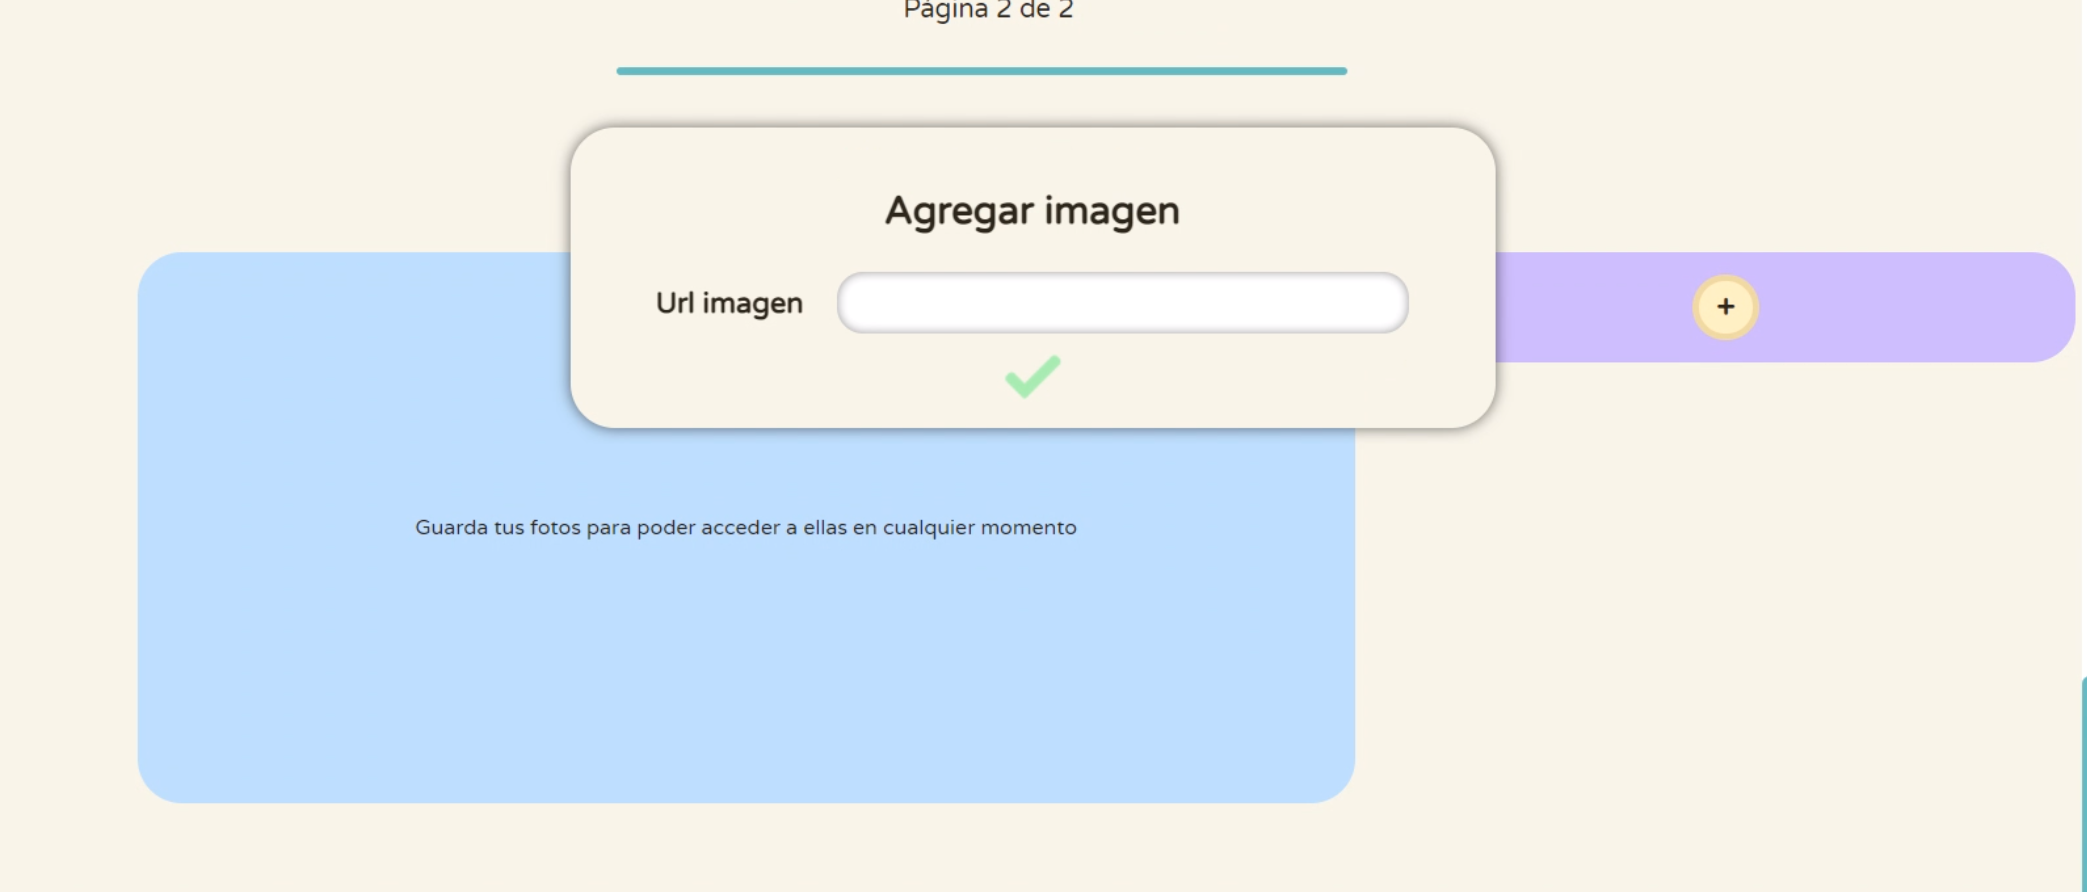
\includegraphics[width=.8\linewidth]{img/cap9/51-anadir-imagen.png}
		\caption{Añadir imagen}
		\label{fig:aniadirimagen}
	\end{minipage}
\end{figure}

Una vez dispongamos de alguna imagen, aparecerá en grande una a la izquierda {(v\'ease la figura~\ref{fig:albumfotos})}, y en caso de tener más de una, podemos seleccionar la imagen que queremos ver en grande, o bien de forma temporal colocando el cursor encima de la imagen, o bien haciendo click para que se mantenga esa selección, que se mostrará algo mas grande que las demás.\\

\figura{0.7}{img/cap9/52-album-fotos-relleno.png}{Álbum con fotos}{fig:albumfotos}{}

Si deseamos borrar alguna foto, es tan sencillo como activar el modo borrado haciendo click en la papelera. Sabremos que estamos en el modo borrado porque cambiará el fondo del menú de morado a rojo {(v\'ease la figura~\ref{fig:borrarimagen})}, y las imágenes temblarán si el cursor se sitúa sobre ellas. Una vez activado, si hacemos click en las imágenes, las borraremos.\\

\figura{0.7}{img/cap9/53-borrar-imagen.png}{Borrar imagen}{fig:borrarimagen}{}

\clearpage

Ahora que hemos visto el funcionamiento del álbum de fotos, podemos pasar a explicar la última herramienta de la página, que sería el catálogo de sueños, al que podremos acceder si hacemos click en el botón ``Sueños" situado en la barra de navegación superior. Esto nos llevará a un catálogo donde podremos ver los sueños que han subido los usuarios {(v\'ease la figura~\ref{fig:catsuenos})}.\\

\figura{0.9}{img/cap9/54-catalogo-suenos.png}{Catálogo sueños}{fig:catsuenos}{}

En cada ítem podremos ver, el nombre de la isla del sueño, su código para poder viajar al mismo, el usuario que ha subido el sueño, así como algunas fotos de la isla que haya querido subir el usuario. En caso de que haya subido más de una (hasta un límite de tres), podemos navegar entre las mismas mediante las flechas situadas a los lados {(v\'ease la figura~\ref{fig:sueno})}.\\

\begin{figure}[!htb]
	\begin{minipage}{0.48\textwidth}
		\centering
		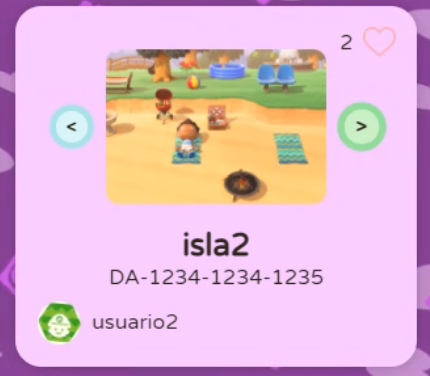
\includegraphics[width=.7\linewidth]{img/cap9/55-sueno.png}
		\caption{Sueño}
		\label{fig:sueno}
	\end{minipage}\hfill
	\begin{minipage}{0.48\textwidth}
		\centering
		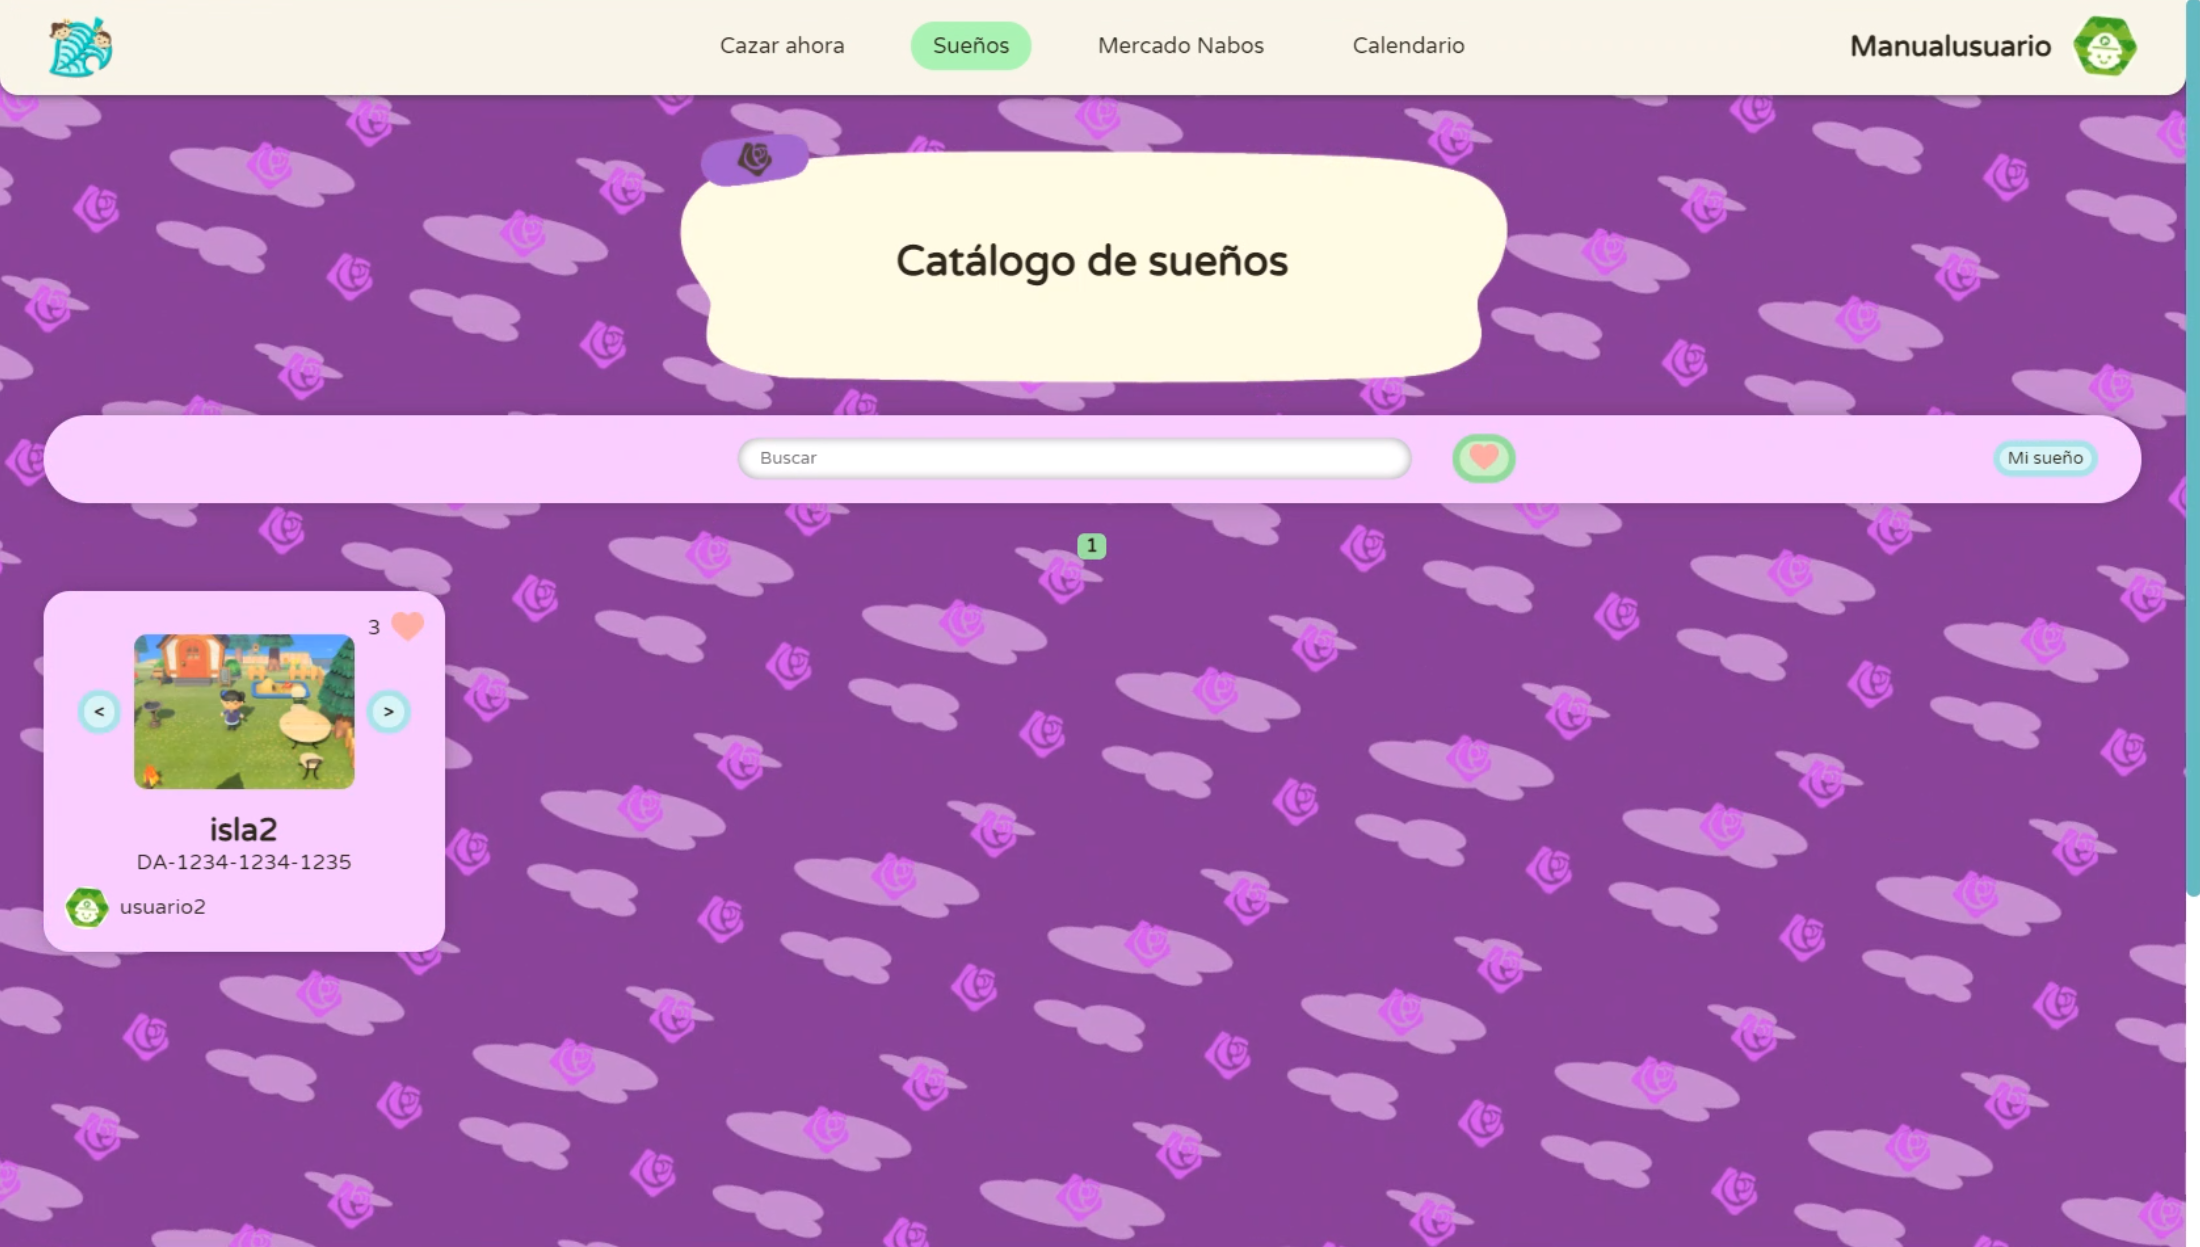
\includegraphics[width=\linewidth]{img/cap9/56-catalogo-sueno-filtro-like.png}
		\caption{Catálogo filtrado}
		\label{fig:catfiltered}
	\end{minipage}
\end{figure}

Además, cada sueño tiene un corazón en la parte superior derecha que indica el número de ``Me gusta" que ha recibido, y haciendo click sobre el podemos darle o quitarle el ``Me gusta". Con esto, no solo podemos indicar que nos ha gustado un sueño, sino que le sirve al usuario como una lista personal de favoritos, ya que en los filtros puede filtrar tanto por el nombre de la isla como por aquellos a los que le haya dado ``Me gusta", {(v\'ease la figura~\ref{fig:catfiltered})}.\\

\clearpage

Si el usuario lo desea, puede subir un sueño haciendo click en el botón ``Mi sueño" que encontrará junto a los filtros a la derecha. Al hacer click, se abrirá un menú tal y como se ve en la imagen {(v\'ease la figura~\ref{fig:crearsueno})}. Aquí podremos introducir el código de nuestro sueño, así como de una a tres imágenes, las cuales podremos seleccionar o deseleccionar haciendo click en ellas. Una vez hallamos rellenado los datos, pulsamos en el botón del check verde para confirmar la creación de nuestro sueño.\\

\figura{0.7}{img/cap9/57-crear-sueno.png}{Crear sueño}{fig:crearsueno}{}

En caso de querer modificar tanto el código como las imágenes, es tan sencillo como volver a hacer click en el botón de ``Mi sueño", y luego modificar los datos. En caso de querer eliminarlo, en el mismo menú podemos hacer click en el icono de la papelera y confirmar nuestra decisión {(v\'ease la figura~\ref{fig:confirmarborrado})}.\\

\figura{0.7}{img/cap9/59-confirmar-borrado.png}{Confirmación borrado}{fig:confirmarborrado}{}